\documentclass{article}

% packages
\usepackage{amsmath, amsthm, thmtools, amsfonts, amssymb, luacode, catchfile, tikzducks, hyperref, ifthen}
\ifcsname c@kobocompile\endcsname
	\usepackage[a5paper, total={1072pt, 1448pt}, margin=10pt, includeheadfoot]{geometry} % set page margins
\else
	\usepackage[a4paper, margin=50pt, includeheadfoot]{geometry}
\fi
\usepackage[shortlabels]{enumitem}
\usepackage[skip=3pt, indent=0pt]{parskip}

% language
\usepackage[bidi=basic, layout=tabular, provide=*]{babel}
\ifcsname c@english\endcsname
	\babelprovide[main, import]{english}
\else
	\babelprovide[main, import]{hebrew}
	\babelprovide{rl}
\fi
%\babelfont{rm}{Libertinus Serif}
\babelfont{rm}[Renderer=Harfbuzz]{Libertinus Serif}
\babelfont{sf}{Libertinus Sans}
\babelfont{tt}{Libertinus Mono}

% style
\AddToHook{cmd/section/before}{\clearpage}	% Add line break before section
\linespread{1.3}
\setcounter{secnumdepth}{0}		% Remove default number tags from sections, this won't do well with theorems
\AtBeginDocument{\setlength{\belowdisplayskip}{3pt}}
\AtBeginDocument{\setlength{\abovedisplayskip}{3pt}}
\graphicspath{ {../images/} }

% operators
\DeclareMathOperator\cis{cis}
\DeclareMathOperator\Sp{Sp}
\DeclareMathOperator\tr{tr}
\DeclareMathOperator\im{Im}
\DeclareMathOperator\re{Re}
\DeclareMathOperator\diag{diag}
\DeclareMathOperator*\lowlim{\underline{lim}}
\DeclareMathOperator*\uplim{\overline{lim}}
\DeclareMathOperator\rng{rng}
\DeclareMathOperator\Sym{Sym}
\DeclareMathOperator\Arg{Arg}
\DeclareMathOperator\Log{Log}
\DeclareMathOperator\dom{dom}
\DeclareMathOperator\supp{Supp}
\DeclareMathOperator\var{Var}
\DeclareMathOperator\cov{Cov}

% commands
%\renewcommand\qedsymbol{\textbf{מש''ל}}
%\renewcommand\qedsymbol{\fbox{\emoji{lizard}}}
\newcommand{\Aa}[0]{\mathcal{A}}
\newcommand{\Bb}[0]{\mathcal{B}}
\newcommand{\CC}[0]{\mathbb{C}}
\newcommand{\Cc}[0]{\mathcal{C}}
\newcommand{\EE}[0]{\mathbb{E}}
\newcommand{\FF}[0]{\mathbb{F}}
\newcommand{\Ff}[0]{\mathcal{F}}
\newcommand{\Ii}[0]{\mathcal{I}}
\newcommand{\Gg}[0]{\mathcal{G}}
\newcommand{\Ll}[0]{\mathcal{L}}
\newcommand{\Mm}[0]{\mathcal{M}}
\newcommand{\NN}[0]{\mathbb{N}}
\newcommand{\Nn}[0]{\mathcal{N}}
\newcommand{\PP}[0]{\mathbb{P}}
\newcommand{\Pp}[0]{\mathcal{P}}
\newcommand{\QQ}[0]{\mathbb{Q}}
\newcommand{\RR}[0]{\mathbb{R}}
\newcommand{\Rr}[0]{\mathcal{R}}
\newcommand{\Ss}[0]{\mathcal{S}}
\newcommand{\TT}[0]{\mathbb{T}}
\newcommand{\Uu}[0]{\mathcal{U}}
\newcommand{\Vv}[0]{\mathcal{V}}
\newcommand{\Ww}[0]{\mathcal{W}}
\newcommand{\ZZ}[0]{\mathbb{Z}}
\newcommand{\acts}[0]{\circlearrowright}
\newcommand{\explain}[2] {
	\begin{flalign*}
		 && \text{#2} && \text{#1}
	\end{flalign*}
}
\newcommand{\maketitleprint}[0]{ \begin{center}
	%\begin{tikzpicture}[scale=3]
	%	\duck[graduate=gray!20!black, tassel=red!70!black]
	%\end{tikzpicture}	
	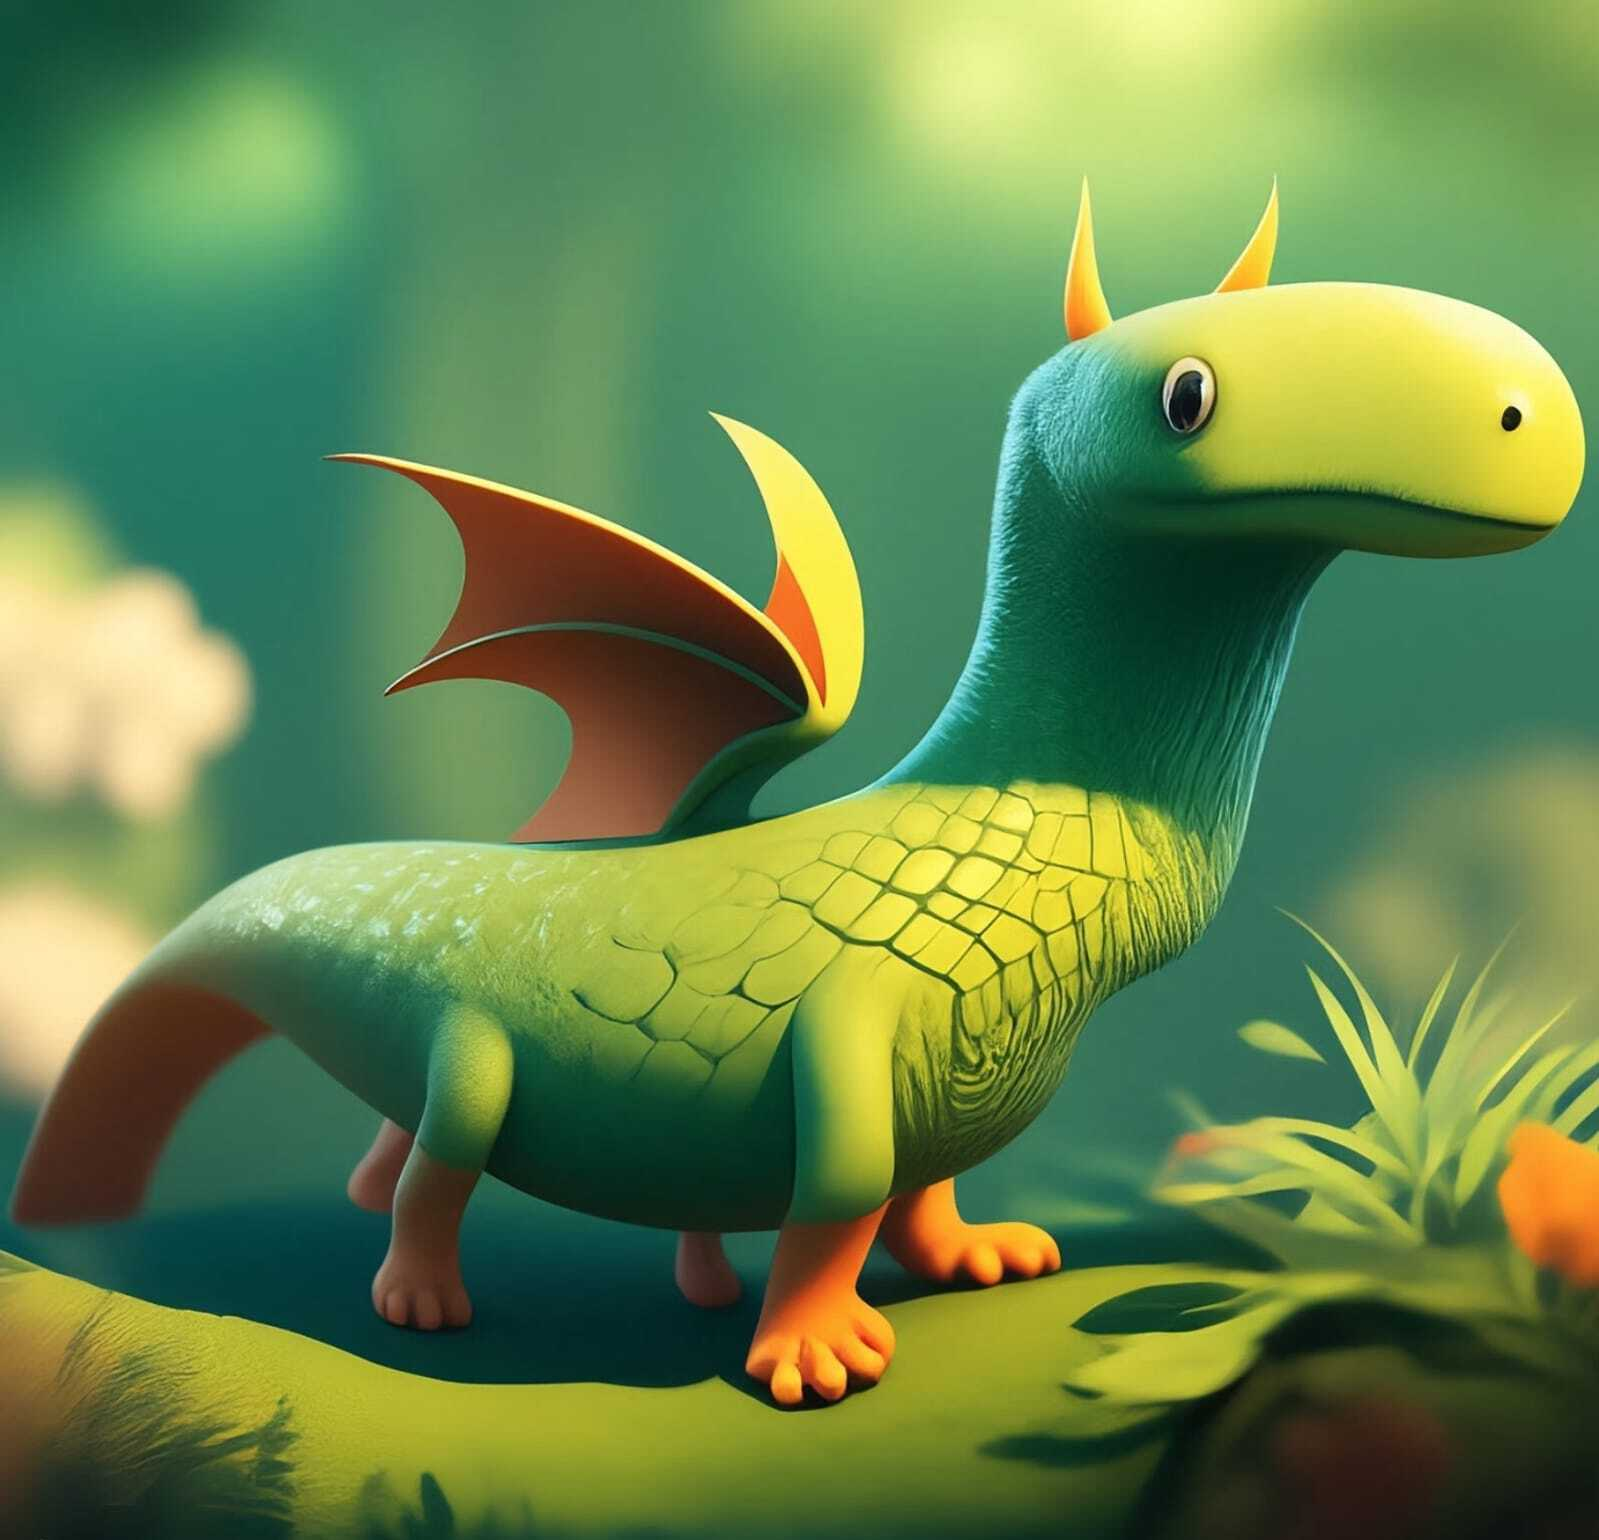
\includegraphics[width=6cm]{cover}
\end{center}
}

% theorem commands
\newtheoremstyle{c_remark}
	{}	% Space above
	{}	% Space below
	{}% Body font
	{}	% Indent amount
	{\bfseries}	% Theorem head font
	{}	% Punctuation after theorem head
	{.5em}	% Space after theorem head
	{\thmname{#1}\thmnumber{ #2}\thmnote{ \normalfont{\text{(#3)}}}}	% head content
\newtheoremstyle{c_definition}
	{3pt}	% Space above
	{3pt}	% Space below
	{}% Body font
	{}	% Indent amount
	{\bfseries}	% Theorem head font
	{}	% Punctuation after theorem head
	{.5em}	% Space after theorem head
	{\thmname{#1}\thmnumber{ #2}\thmnote{ \normalfont{\text{(#3)}}}}	% head content
\newtheoremstyle{c_plain}
	{3pt}	% Space above
	{3pt}	% Space below
	{\itshape}% Body font
	{}	% Indent amount
	{\bfseries}	% Theorem head font
	{}	% Punctuation after theorem head
	{.5em}	% Space after theorem head
	{\thmname{#1}\thmnumber{ #2}\thmnote{ \text{(#3)}}}	% head content

\ifcsname c@english\endcsname
	\theoremstyle{plain}
	\newtheorem{theorem}{Theorem}[section]
	\newtheorem{lemma}[theorem]{Lemma}
	\newtheorem{proposition}[theorem]{Proposition}
	\newtheorem*{proposition*}{Proposition}
	%\newtheorem{corollary}[theorem]{אין חלופה עברית}

	\theoremstyle{definition}
	\newtheorem{definition}[theorem]{Definition}
	\newtheorem*{definition*}{Definition}
	\newtheorem{example}{Example}[section]
	\newtheorem{exercise}{Exercise}[section]

	\theoremstyle{remark}
	\newtheorem*{remark}{Remark}
	\newtheorem*{solution}{Solution}
	\newtheorem{conclusion}[theorem]{Conclusion}
	\newtheorem{notation}[theorem]{Notation}
\else
	\theoremstyle{c_plain}
	\newtheorem{theorem}{משפט}[section]
	\newtheorem{lemma}[theorem]{למה}
	\newtheorem{proposition}[theorem]{טענה}
	\newtheorem*{proposition*}{טענה}
	%\newtheorem{corollary}[theorem]{אין חלופה עברית}

	\theoremstyle{c_definition}
	\newtheorem{definition}[theorem]{הגדרה}
	\newtheorem*{definition*}{הגדרה}
	\newtheorem{example}{דוגמה}[section]
	\newtheorem{exercise}{תרגיל}[section]

	\theoremstyle{c_remark}
	\newtheorem*{remark}{הערה}
	\newtheorem*{solution}{פתרון}
	\newtheorem{conclusion}[theorem]{מסקנה}
	\newtheorem{notation}[theorem]{סימון}
\fi

% Questions related commands
\newcounter{question}
\setcounter{question}{1}
\newcounter{sub_question}
\setcounter{sub_question}{1}

\ifcsname c@english\endcsname
	\newcommand{\question}[1][0]{
		\ifthenelse{#1 = 0}{}{\setcounter{question}{#1}}
		\section{Question \arabic{question}}
		\addtocounter{question}{1}
		\setcounter{sub_question}{1}
	}

	\newcommand{\subquestion}[1][0]{
		\ifthenelse{#1 = 0}{}{\setcounter{sub_question}{#1}}
		\subsection{Part \alph{sub_question}}
		\addtocounter{sub_question}{1}
	}
\else
	\newcommand{\question}[1][0]{
		\ifthenelse{#1 = 0}{}{\setcounter{question}{#1}}
		\section{שאלה \arabic{question}}
		\addtocounter{question}{1}
		\setcounter{sub_question}{1}
	}

	\newcommand{\subquestion}[1][0]{
		\ifthenelse{#1 = 0}{}{\setcounter{sub_question}{#1}}
		\subsection{סעיף \localecounter{letters.gershayim}{sub_question}}
		\addtocounter{sub_question}{1}
	}
\fi

% import lua and start of document
\directlua{common = require ('../common')}

\GetEnv{AUTHOR}

% headers
\author{\AUTHOR}
\date\today

\title{פתרון מטלה 03 --- מבנים אלגבריים 1 (80445)}

\begin{document}
\maketitle
\maketitleprint{}

\Question{}
\Subquestion{}
תהי $G$ חבורה ועבור $g \in G$ נגדיר $\varphi_g : G \to G$ על־ידי $\varphi_g(h) = g h g^{-1}$. \\*
נוכיח ש־$\varphi_g$ הוא אוטומורפיזם וש־$\phi : G \to Aut(G)$ המוגדר על־ידי $\phi(g) = \varphi_g$ הוא הומומורפיזם.
\begin{proof}
	נוכיח תחילה ש־$\varphi_g$ היא הומומורפיזם. \\*
	נראה כי
	\[
		\forall x, y \in G, \varphi_g(x y)
		= g x y g^{-1}
		= g x \overset{=e_G}{(g^{-1} g)} y g^{-1}
		= \varphi_g(x) \cdot \varphi_g(y)
	\]
	ומצאנו כי התנאי ההכרחי להומומורפיזם מתקיים. \\*
	באותו אופן גם $\varphi_{g^-1}$ הוא הומומורפיזם ונשים לב שמתקיים
	\[
		\forall x \in G, (\varphi_{g^-1} \circ \varphi_g)(x) = g^{-1}g x g^{-1} g = x, \qquad
		(\varphi_g \circ \varphi_{g^-1})(x) = g g^{-1} x g g^{-1} = x
	\]
	ומצאנו כי התנאי ההכרחי לאיזומורפיה מתקיים ובהתאם $\varphi_g : G \xrightarrow{\sim} G$.

	מצאנו כי $\varphi_g$ הוא אוטומורפיזם לכל $g \in G$, וכן כי $\varphi_{g^{-1}}$ אוטומורפיזם הופכי לה. \\*
	נראה כי גם
	\[
		\forall x \in G : \phi(g h)(x)
		= \varphi_{gh}(x)
		= gh x h^{-1} g^{-1}
		= g (h x h^{-1}) g^{-1}
		= (\varphi_g \circ \varphi_h)(x)
	\]
	ומצאנו כי התנאי להומומורפיזם מתקיים ובהתאם $\phi : G \xrightarrow{\sim} Aut(G)$.
\end{proof}

\Subquestion{}
נוכיח שלכל $g \in G$ וכל תת־חבורה $H \le G$ מתקיים $g H g^{-1} \le G$.
\begin{proof}
	ראינו כי $\varphi_g$ היא אוטומורפיזם ולכן מתקיימות התכונות:
	\begin{enumerate}
		\item קיום נייטרלי: $e \in H \implies g e g^{-1} = e \in gHg^{-1}$.
		\item סגירות לכפל: הוכחנו בסעיף הקודם.
		\item קיום הופכי: $\forall x \in G: \varphi_g(x) \varphi_g(x^{-1}) = \varphi_g(x^{-1}) \varphi_g(x) = \varphi_g(e) = e$
	\end{enumerate}
	ומצאנו כי זוהי תת־חבורה.
\end{proof}

\Subquestion{}
תהי קבוצה $X$ ופעולה $\cdot : G \times X \to X$ ונוכיח שלכל $x, y \in X$, אם קיים $g \in G$ כך ש־$y = gx$ אז $G_y = g G_x g^{-1}$.
\begin{proof}
	נניח כי התנאים מתקיימים, נבחין כי $G_x = \{ h \in G \mid h x = x \}$. \\*
	נבחר $h \in G_x$ ונקבל
	\[
		y = g(hx) = (gh) x \iff h^{-1} g^{-1} y = x \iff g h^{-1} g^{-1} y = gx = y \iff h^{-1} \in G_y \iff h \in G_y
	\]
	ומצאנו כי $G_y = g G_x g^{-1}$
\end{proof}

\Question{}
\Subquestion{}
יהי $\tau = (a_1\ a_2 \dots a_k) \in S_n$ מחזור ו־$\sigma \in S_n$. נוכיח כי
\[
	\sigma (a_1\ a_2 \dots a_k) \sigma^{-1} = (\sigma(a_1)\ \sigma(a_2) \dots \sigma(a_k))
\]
\begin{proof}
	יהי $a_m$ כך ש־$1 \le m < k$. \\*
	אז $(\sigma \circ \tau \circ \sigma^{-1})(\sigma(a_m)) = \sigma(\tau(a_m)) = \sigma(a_{m + 1})$. \\*
	עוד נראה כי $(\sigma \circ \tau \circ \sigma^{-1})(\sigma(a_k)) = \sigma(a_1)$. \\*
	עבור $a_m$ כאשר $k < m \le n$ נקבל $(\sigma \circ \tau \circ \sigma^{-1})(\sigma(a_m)) = \sigma(a_m)$. \\*
	לסיכום מצאנו כי $(\sigma \circ \tau \circ \sigma^{-1})(\sigma(a_m)) = \sigma(a_{m + 1})$ עבור $m \le k$ ו־$(\sigma \circ \tau \circ \sigma^{-1})(\sigma(a_m)) = \sigma(a_m)$ עבור שאר ערכי $m$ ובהתאם מתקיים
	\[
		\sigma (a_1\ a_2 \dots a_k) \sigma^{-1} = (\sigma(a_1)\ \sigma(a_2) \dots \sigma(a_k))
	\]
\end{proof}

\Subquestion{}
נוכיח ששתי תמורות הן צמודות אם ורק אם הפירוק שלהן למחזורים מכיל מספר זהה של מחזורים מכל אורך.
\begin{proof}
	\textbf{כיוון ראשון:}
	נניח ששתי חבורות $\tau, \phi$ צמודות, לכן קיים $\sigma \in S_n$ כך ש־$\tau = \sigma \phi \sigma^{-1}$. \\*
	נוכל לפרק את $\phi = \phi_1\circ\cdots \circ \phi_k$ ל־$k$ מחזורים שונים. \\*
	נבחין כי $Id = \sigma \sigma^{-1} = \sigma^{-1} \sigma$ וננצל עובדה זאת כדי לראות שמתקיים
	\[
		\tau
		= \sigma \circ \phi \circ \sigma^{-1}
		= \sigma \circ \phi_1 \circ \phi_2 \circ \cdots \circ \phi_k \circ \sigma^{-1}
		= \sigma \circ \phi_1 \sigma^{-1} \sigma \circ \phi_2\sigma^{-1} \sigma \circ \cdots \circ \sigma^{-1} \sigma\phi_k \circ \sigma^{-1}
	\]
	לכן $\tau$ הוא הרכבה של אוסף תמורות מהצורה $\sigma \phi_i \sigma^{-1}$ ובסעיף הקודם הראינו כי אלו מחזורים משמרי אורך, ומצאנו כי לשתי התמורות $\tau$ ו־$\phi$ פירוק למחזורים זהה.

	\textbf{כיוון שני:}
	נניח כי לשתי חבורות $\tau, \phi$ יש פירוק למחזורים זהה, $\tau = \tau_1 \circ \cdots \circ \tau_l, \phi = \phi_1 \circ \cdots \circ \phi_l$ \\*
	נגדיר כי $\tau_i, \phi_i$ כאשר $1 \le i \le l$ מחזורים באורך זהה בין שתי התמורות. לכן
	\[
		\phi_i = (a_1\ a_2 \dots a_k), \qquad
		\tau_i = (b_1\ b_2 \dots b_k)
	\]
	נגדיר תמורה חדשה $\sigma_i \in S_n$ על־ידי $\sigma(a_j) = b_j$ לכל $1 \le j \le k$. \\*
	מסעיף א' נקבל מיידית
	\[
		\sigma_i \phi_i \sigma_i^{-1} = \tau_i
	\]
	נגדיר $\sigma = \sigma_1 \circ \cdots \circ \sigma_l$. נבחין כי המחזורים הם זרים אחד לשני, שכן מקורותיהם מוגדרים על־ידי מחזורים זרים של $\tau$. \\*
	נראה כי
	\[
		\sigma \phi_1 \sigma^{-1} \circ
		\sigma \phi_2 \sigma^{-1} \circ
		\cdots
		\sigma \phi_l \sigma^{-1}
		= \tau
		= \sigma \phi_1 \cdots \phi_l \sigma^{-1}
		= \sigma \phi \sigma^{-1}
	\]
	וקיבלנו כי הטענה נכונה.
\end{proof}

\Question{}
יהי $\sigma = (1\ 2\ 3\ 4), \tau = (2\ 3)(4\ 1) \in D_4 \le S_4$.

\Subquestion{}
נחשב את המרכז של $\sigma, \tau$ ב־$D_4$.

נתחיל בחישוב $C_{D_4}(\sigma)$. בשאלה 2 מצאנו כי עבור $\phi$ תמורה אז $\phi \sigma \phi^{-1} = \sigma \iff (\phi(1)\ \phi(2)\ \phi(3)\ \phi(4)) = (1\ 2\ 3\ 4)$. \\*
דהינו על $\phi$ לשמר את סדר המחזור, לכן נוכל לבחור רק $\phi = \sigma^k$ עבור $0 \le k < 4$. \\*
לכן $C_{D_4}(\sigma) = \{ Id, \sigma, (1\ 3)(2\ 4), (1\ 4)(2\ 3) \}$. \\*
נחשב עתה את $C_{D_4}(\tau)$. במטלה הקודמת מצאנו כי $\sigma^k \tau \sigma^{-k} = \tau \sigma^{-2k}$ ולכן רק עבור $k = 2$ נקבל $\sigma^2 \tau \sigma^{-2} = \tau$. \\*
נקבל גם $\tau \sigma^k \tau {(\tau \sigma^k)}^{-1} = \tau \sigma^k \tau \tau \sigma^{n - k} = \tau$.
וקיבלנו כי $C_{D_4}(\tau) = \{ Id, \tau, \tau \sigma, \tau \sigma^2, \tau \sigma^3, \sigma^2\}$.

\Subquestion{}
נחשב את מחלקות הצמידות של $D_4$.

בסעיף הקודם למעשה מצאנו שיוך של כל איבר ב־$D_4$ למרכז כלשהו, ולכן מחלקות הצמידות הן
\[
	\{ \{ Id, \sigma, \sigma^2, \sigma^3 \},
	\{ Id, \tau, \tau \sigma, \tau \sigma^2, \tau \sigma^3, \sigma^2\}
	\}
\]

\Subquestion{}
נמצא שני איברים שאינם צמודים ב־$D_4$ אבל כן ב־$S_4$.

נבחר את $\tau, \sigma^2$:
\[
	\sigma^2 = (1 3)(2 4), \tau = (1 4)(2 3)
\]
נגדיר $\phi = (3 4)$ על־פי שאלה 2 ונקבל $\phi \sigma^2 \phi^{-1} = \tau$, אבל $\phi \not\in D_4$.

\Question{}
נגדיר את הפעולה הבאה של $S_n$ על ${[n]}^2$: לכל $\sigma \in S_n$ ו־$(i, j) \in {[n]}^2$ נגדיר $\sigma . (i, j) = (\sigma(i), \sigma(j))$. \\*
נחשב את המסלולים של הפעולה של $S_n$ על ${[n]}^2$.

בהרצאה מצאנו כי הפעולה של $S_n$ מעל $[n]$ היא טרנזיטיבית, דהינו קיים רק מסלול אחד בין כלל האיברים. \\*
נטען כי בפעולה שהגדרנו זה עתה ישנם שני מסלולים בלבד:
\begin{enumerate}
	\item $O((1, 1)) = \{ (i, i) \in {[n]}^2 \mid i \in [n]\}$. \\*
		יהי $i, j \in [n]$ כך ש־$i \ne j$. ונגדיר $\sigma = (i\ j)$, לכן $\sigma . (i, i) = (j, j)$ ומצאנו כי מסלול זה נכון.
	\item $O((i, j)) = \{ (a, b) \in {[n]}^2 \mid a \ne b, 0 \le a, b < n \}$. \\*
		יהי $i, j$ כך ש־$i \ne j$, ויהיו $a, b$ כך שגם $a \ne b$, ו$i, j, a, b \in [n]$, אז נגדיר $\sigma = (i\ a)(j\ b)$, ומצאנו כי גם זה אכן מסלול.
\end{enumerate}
נשים לב שכל תמורה היא חד־חד ערכית, ולכן לא יתכן ש־$a = b$ ולכן אין מסלול בין $(i, j) \to (a, a)$, ובאופן דומה כמובן אין תמורה $(a, a) \to (i, j)$ כאשר $i \ne j$. \\*
לסיכום ישנם שני מסלולים שונים לפעולה, $O(0, 0), O(0, 1)$ בלבד.

\Question{}
\Subquestion{}
תהי $G$ חבורה אבלית ו־$H, K \le G$ תת־חבורות, כך ש־$H \cap K = \{ e \}$ ו־$H \cdot K = G$. \\*
נוכיח ש־$H \times K \xrightarrow{\sim} G$.
\begin{proof}
	נגדיר פונקציה $\phi : H \times K \to G$ על־ידי $\phi(h, k) = h \cdot k$. אז
	\[
		\phi(h_1 h_2, k_1 k_2)
		= (h_1 h_2)(k_1 k_2)
		\overset{\text{אבליות}}{=} h_1 (h_2k_1) k_2
		= (h_1 k_1) (h_2 k_2)
		= \phi(h_1, k_1) \phi(h_2, k_2)
	\]
	ומצאנו כי $\phi$ הומומורפיזם. \\*
	נגדיר $\varphi : G \to H \times K$ על־ידי שימוש בנתון $HK = G$, ידוע כי $\forall G \in G \exists h \in H, k \in K : g = hk$ ולכן נגדיר $\varphi(g) = hk$. 
	לכן גם $\forall g_1, g_2 \in G \exists h_1, h_2 \in H, k_1, k_2 \in K : g_1 = h_1 k_1, g_2 = h_2 k_2, \varphi(g_1 g_2) = \varphi(h_1 (k_1 h_2) k_2) = \varphi((h_1 h_2) e \cdot (k_1 k_2) e) = \varphi(h_1h_2) \varphi(k_1k_2)$.
	ונסיק כי $\varphi$ הומומורפיזם, ונשים לב ש־$\phi \circ \varphi = Id, \varphi \circ \phi = Id$ ולכן $\varphi^{-1} = \phi$ ונובע ש־$G$ איזומורפית ל־$H \times K$.
\end{proof}

\Subquestion{}
נמצא חבורה $G$ ושתי תת־חבורות שלה $H, K \le G$ כך ש־$H \cdot K$ היא לא תת־חבורה.

נגדיר $G = S_3, H = \{e, (1\ 2) \}, K = \{e, (2\ 3)\}$. 
נשים לב ששתי תת־החבורות מוגדרות היטב, שכן לכל איבר יש הופכי, ושתי תת־החבורות אכן סגורות (באופן ריק) לכפל.
נחשב ונקבל $H \cdot K = \{ e, (1\ 2), (2\ 3), (1\ 3\ 2)\}$. \\*
אנו רואים כי $(1\ 3\ 2) \in H \cdot K$ אבל ${(1\ 3\ 2)}^{-1} = (2\ 3\ 1) \notin H \cdot K$, דהינו הסגירות להופכי לא מתקיימת ב־$H \cdot K$ ולכן זוהי לא תת־חבורה.

\end{document}
